\documentclass{beamer}
 
%presentation pre-amble
%The idea behind this file is that it will be used to store all the maths-related macros that I concoct; so that I can import all the commands by \input{this file} in the preamble of any file that I want to use them in.
%This should make the top-level files look a lot cleaner, and the preamble much shorter!

\usepackage{amssymb}
\usepackage{amsmath}
%\usepackage{mathtools}

%begin the macros via newcommand. Try to group them up reasonably!

%standard sets
\newcommand{\naturals}{\mathbb{N}}			%natural numbers
\newcommand{\integers}{\mathbb{Z}}			%integers
\newcommand{\rationals}{\mathbb{Q}}			%rational numbers
\newcommand{\reals}{\mathbb{R}}				%real numbers
\newcommand{\complex}{\mathbb{C}}			%complex numbers

%brackets and norms
\newcommand{\bracs}[1]{\left( #1 \right)}				%encloses input in brackets
\newcommand{\sqbracs}[1]{\left[ #1 \right]}				%encloses input in square brackets
\newcommand{\clbracs}[1]{\left\{ #1 \right\}}			%encloses input in curly bracers
\newcommand{\abs}[1]{\lvert #1 \rvert}					%absolute value
\newcommand{\norm}[1]{\lvert\lvert #1 \rvert\rvert}		%norm 

%function sets
\newcommand{\smooth}[1]{C^{\infty}\bracs{#1}}							%smooth functions
\newcommand{\ltwo}[2]{L^{2}\bracs{#1,\mathrm{d}#2}}						%general L^2 space
\newcommand{\gradSob}[2]{H^1_\mathrm{grad}\bracs{#1, \mathrm{d}#2}}		%gradient Sobolev space
\newcommand{\curlSob}[2]{H^1_\mathrm{curl}\bracs{#1, \mathrm{d}#2}}		%curl Sobolev space
\newcommand{\kSob}[2]{H^1_{k,\mathrm{curl}}\bracs{#1, \mathrm{d}#2}}	%k-curl Sobolev space
\newcommand{\supp}{\mathrm{supp}}										%support of a function

%grad and curl sets
\newcommand{\gradZero}[2]{\mathcal{G}_{ #1, \mathrm{d}#2}\bracs{0}}		%gradients of zero for domain #1 with measure #2
\newcommand{\curlZero}[2]{\mathcal{C}_{ #1, \mathrm{d}#2}\bracs{0}}	%curls of zero for domain #1 with measure #2
\newcommand{\kcurlZero}[2]{\mathcal{C}_{ #1, \mathrm{d}#2}^{(k)}\bracs{0}}	%k-curls of zero for domain #1 with measure #2

%derivatives and grad-like symbols
\newcommand{\diff}[2]{\dfrac{\mathrm{d}#1}{\mathrm{d}#2}}			%complete derivative d#1/d#2
\newcommand{\pdiff}[2]{\dfrac{\partial #1}{\partial #2}}			%partial derivative p#1/p#2
\newcommand{\ddiff}[2]{\dfrac{\mathrm{d}^2 #1}{\mathrm{d}^2 #2}}	%2nd deriv
\newcommand{\grad}{\nabla}											%grad operator
\newcommand{\curl}[1]{\grad^{(#1)}\wedge}							%curl with superscript #1
\newcommand{\kcurl}[1]{\grad_{#1}^{(k)}\wedge}						%k-curl with measure subscript #1

%displaying integrals
\newcommand{\integral}[3]{\int_{#1}#2 \ \mathrm{d}#3}			%integral, domain #1, integrand #2, measure #3
\newcommand{\md}{\ \mathrm{d}}									%differential d

%convergence
%\newcommand{\lconv}[1]{\xrightarrow{#1}}							%convergence with #1 above the rightarrow - requires mathtools
\newcommand{\lconv}[1]{\overset{#1}{\longrightarrow}}				%convergence with #1 above the rightarrow
\newcommand{\toInfty}[1]{ \ \text{as} \ #1 \rightarrow\infty}		%writes out "as #1 tends to infty"

%notation and variable use throughout the file
\renewcommand{\vec}[1]{\mathbf{#1}}				%vectors are bold, not overline arrow
\newcommand{\recip}[1]{\frac{1}{#1}}			%fast reciprocal as a fraction

\newcommand{\dddom}{\widetilde{\Omega}}			%3D domain notation
\newcommand{\ddom}{\Omega}						%2D domain notation
\newcommand{\dddmes}{\widetilde{\mu}}			%3D measure
\newcommand{\ddmes}{\mu}						%2D measure

\newcommand{\graph}{\mathbb{G}}					%graph variable
%Preamble file for all presentation styles but not including maths formatting!

\usepackage[utf8]{inputenc}

\usepackage{graphicx}
\usepackage{subcaption}
\usepackage{tikz}
\usetikzlibrary{arrows}

\usetheme{Madrid}
\usecolortheme{default}
 
%removes figure prefix from captions
\setbeamertemplate{caption}{\raggedright\insertcaption\par}

%sets the directory for image files - note: this assumes the file structure as of 14-10-2019
\graphicspath{{../Diagrams/Diagram_PDFs/} {../Images/}}

\usepackage{soul} %strikethrough text via \st
\usepackage{graphicx}
\graphicspath{{../Diagrams/Diagram_PDFs/}, {./PSS_Diagrams/}}
\usepackage{ifthen}

\usepackage{tikz}
\newcommand{\cross}[2]{
\begin{scope}[shift={#1}]
	\filldraw[black!30!white] (-#2,-#2) -- (-#2,-1) -- (#2,-1) -- (#2,-#2) -- (1,-#2) -- (1,#2) -- (#2,#2) -- (#2,1) -- (-#2,1) -- (-#2,#2) -- (-1,#2) -- (-1,-#2) -- cycle;
\end{scope}
}
\newcommand{\eps}{\varepsilon}

%Information to be included in the title page
\title{Motivation of and Considerations for Singular-Structure Problems}
\author{William Graham}
\institute{SAMBa Conference 2020}
\date{\today}
 
\begin{document}
 
\frame{\titlepage}

\begin{frame}
	\begin{columns}
		\begin{column}{0.55\textwidth}
				\begin{figure}
					\centering
					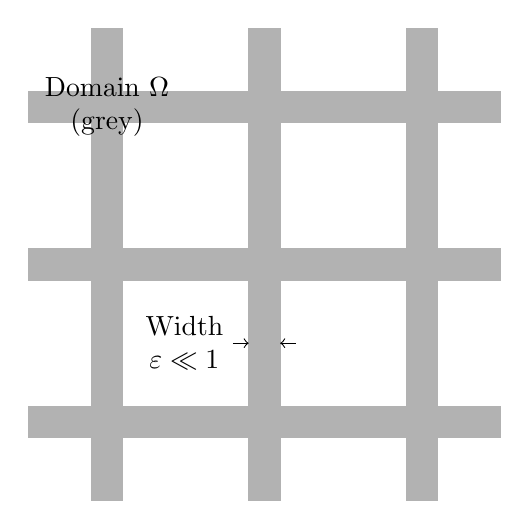
\begin{tikzpicture}
							\foreach \y in {0, ..., 1}
								\foreach \x in {0, ..., 1}
									\cross{(\x*2,\y*2)}{0.2}
									\cross{(-\x*2,-\y*2)}{0.2}
									\cross{(\x*2, -\y*2)}{0.2}
									\cross{(-\x*2,\y*2)}{0.2}
									; %end for \x
								] %end for \y
								
								%domain label
								\node[align=center] at (-2.,2.) {Domain $\Omega$ \\ (grey)};
								%governing equation on domain
								%\node[align=center] at (0,0) {$-\nabla^2 u = \omega^2 u$};
								%boundary conditions
								%\node[align=center] at (1,1) {$\pdiff{u}{\mathbf{n}}\big\vert_{\partial\Omega}=0$};
								%thickness
								\draw[->] (-0.4,-1) -- (-0.2,-1);
								\draw[->] (0.4,-1) -- (0.2,-1);
								\node[align=center, anchor=east] at (-0.4,-1) {Width \\ $\eps\ll 1$};
					\end{tikzpicture}
				\end{figure}
		\end{column}
		\begin{column}{0.35\textwidth}
			\begin{block}{Thin Domains}
				\begin{itemize}
					\item ``Width" $\eps\ll 1$.
					\item PDEs are computationally solvable, analytically challenging.
				\end{itemize}
			\end{block}
			\begin{block}{The Idea}
				Can we provide an \emph{approximate} model?
			\end{block}
		\end{column}
	\end{columns}
\end{frame}

\begin{frame}
	\frametitle{Singular-Structures}
	
	\begin{figure}
		\centering
		\includegraphics[scale=0.5]{Domain_Illustrations.pdf}
	\end{figure}
	
	The domain on the right is a ``singular structure" - it has \emph{no width}, or \emph{no area}.
	\begin{block}{The Question}
		Can we provide a coherent notation of a ``PDE" on a singular structure domain, and can we make progress solving it analytically?		 
	\end{block}
	
\end{frame}

\begin{frame}
	\frametitle{Considerations}
	
	\begin{block}{Main Issue}
		Our singular-structure is a 1D object in a 2D space!
	\end{block}
	The end result is a ``weak" formulation, which uses new concepts of ``area" and ``gradient":
	\begin{figure}
		\centering
		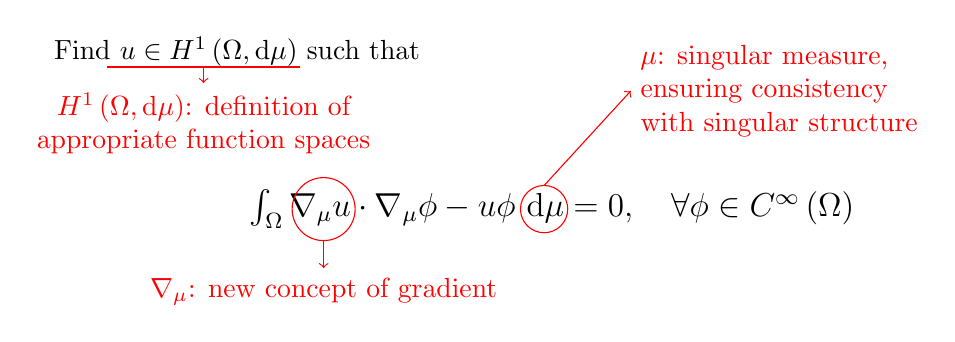
\begin{tikzpicture}
			\node[align=center] at (-4,2) {Find $u\in H^1\bracs{\ddom,\mathrm{d}\mu}$ such that};
			\node[align=center] at (0,0) {\large $\integral{\ddom}{\grad_{\mu}u \cdot \grad_{\mu}\phi - u\phi}{\mu} = 0, \quad \forall \phi\in\smooth{\ddom}$};
			
			\draw[red] (-0.1,0) circle (0.3);
			\draw[red, ->] (-0.1,0.3) -- (1,1.5) node[anchor=west, align=left] {$\mu$: singular measure, \\ ensuring consistency \\ with singular structure};
			
			\draw[red] (-2.9,0) circle (0.4);
			\draw[red, ->] (-2.9,-0.4) -- (-2.9,-0.75) node[anchor=north] {$\grad_{\mu}$: new concept of gradient};
			
			\draw[red, thick] (-5.65,1.8) -- (-3.2,1.8);
			\draw[red, ->] (-4.425, 1.8) -- (-4.425,1.6) node[anchor=north, align=center] {$H^1\bracs{\ddom,\mathrm{d}\mu}$: definition of \\ appropriate function spaces};
		\end{tikzpicture}
	\end{figure}

	Forgetting the $\mu$'s everywhere, compare this to the weak formulation of
	\begin{align*}
		-\grad^2 u - u = 0, \quad \text{on a thin domain}.  
	\end{align*}
\end{frame}

\end{document}
